%%%%%%%%%%%%%%%%%%%%%%%%%%%%%%%%%%%%%%%%%%%%%%%%%%%%%%%%%%%%%%%%%%%%%%
% How to use writeLaTeX: 
%
% You edit the source code here on the left, and the preview on the
% right shows you the result within a few seconds.
%
% Bookmark this page and share the URL with your co-authors. They can
% edit at the same time!
%
% You can upload figures, bibliographies, custom classes and
% styles using the files menu.
%
%%%%%%%%%%%%%%%%%%%%%%%%%%%%%%%%%%%%%%%%%%%%%%%%%%%%%%%%%%%%%%%%%%%%%%

\documentclass[12pt]{article}

\usepackage{sbc-template}
\usepackage{hyperref}
\usepackage{graphicx,url}
\usepackage{graphicx,url}
\usepackage{subfigure}
\usepackage{float}
%\usepackage[brazil]{babel}   
\usepackage[utf8]{inputenc}  

     
\sloppy

\title{Keylogger e Screenlogger}

\author{André Filipe Pereira de Almeida}


\address{Sistemas de Informação -- Universidade Federal dos Vales do Jequitinhonha e Mucuri
  \\(UFVJM)\\
}

\begin{document} 

\maketitle

\begin{abstract}
  This work aims to present what it is and how it works as \textit{keyloggers} and \textit {Screenloggers} tools, which can be used in legal or illegal ways, if used as a form of execution they can be extremely harmful and cause huge damages and losses, since its use is legally foreseen for controversies because although they can be used it does not mean that people will accept it or whoever uses it will be seen with good eyes.
\end{abstract}
     
\begin{resumo} 
  Esse trabalho tem como objetivo apresentar o que é e como funciona as ferramentas de \textit{keyloggers} e \textit{Screenloggers}, que podem ser utilizadas de formas legais ou ilegais, se utilizadas como forma de ataques podem ser extremamente prejudiciais e causar danos e prejuízos gigantes, já seu uso legalmente previsto á controvérsias pois apesar de poderem ser usadas não significa que as pessoas vão aceitar ou quem utilizar será visto com bons olhos.   
\end{resumo}


\section{Introdução}
O que é um \textit{keylogger}?

A palavra é uma abreviação de um termo inglês chamado \textit{keystroke logger} (registrador de digitação) essa ferramenta tem como objetivo monitorar tudo que você digita, pode ser tanto um software como um hardware, ele pode ser um programa instalado ou algum dispositivo conectado ao pc ou teclado.

Essa ferramenta é um tipo de \textit{spyware} e permite que o criminoso roube informações valiosas como senhas, logins, conversas completas, sites que acessou, aplicativos usados e etc.

Mas diferente do que muitos acreditam, os \textit{keyloggers} são lícitos, isso porque eles não foram projetados para roubar dados por isso existe um grande quantidade disponível na internet para baixar, eles são usados por empresas para vigiar seus funcionários, pais que querem saber o que os filhos fazem na internet ou companheiros que querem descobrir uma traição.

Como é uma ferramenta não ilegal o que você faz com ela é que importa, por exemplo se estiver na politica de segurança da empresa o técnico responsável pode instalar nas maquinas e por mais que os colaboradores não gostem é licito, o grande problema é quando caem em mãos erradas pois as informações coletadas podem causar enormes prejuízos pessoais e corporativos, é muito importante que não deixe o computador desbloqueado em qualquer lugar e tenha cuidado com os sites acessados pois os \textit{keyloggers} se espalham principalmente na internet como parte dos cavalos de troia que oferecem uma ferramenta e acaba contendo um malware que é instalado na maquina e rodado em segundo plano

Basicamente existem 3 tipos de \textit{keyloggers} que são:

\begin{itemize}
  \item \textbf{Driver ou Kernel keylogger:} ele atua como se fosse um driver onde pega informações diretamente dos periféricos de entrada, mouse ou teclado por exemplo, ou seja eles não podem recuperar dados de preenchimento automático como senhas, e-mails e endereço. 
  \item \textbf{Softwares que utilizam a funcionalidade “hooking”:} estes são mais complexos e além de uma biblioteca DDL para interpretação também possuem um programa executável que viabiliza sua ação, por meio da função SetWindowsHookEx() do windows consegue captar dados.
  \item \textbf{Hardware keyloggers:} esse tipo como o nome da deixa claro são peças físicas colocas entre o teclado e a CPU e não podem ser detectados por antivírus. 
\end{itemize}

As formas de identificar um keylogger são bem comuns, verificar o gerente de tarefas do windows, olhar o registro do firewall e escaneamento com antivírus e para os que são hardware é mais fácil de identificar pois pode ser um pendrive novo plugado.

Os \textit{Screenloggers} são ferramentas muito iguais ao \textit{keylogger} porém elas capturam a posição do mouse na tela e captura de imagens da tela então mesmo que o usuário utilize um teclado virtual se a maquina estiver infectada as informações serão roubadas da mesma forma.

\section{Material e métodos} \label{sec:firstpage}
Como o enfoque do trabalho é para ser voltado pra mobile realizei uma pesquisa sobre aplicativos com esse tipo de função e a grande maioria deles é pago e são bastante caros, alguns possuem versão de teste e os que são gratuitos tem vários problemas, acabei chegando no \textbf{Snoopza} que é um aplicativo para android (\url{https://snoopza.com/br}). 

Ele é pago e custa \$14,95 por mês ou \$99,95 em assinatura anual, a sua versão gratuita possui as funções de rastreio de chamadas, histórico de SMS, rastreio de histórico da internet e rastreio de geolocalização; Já sua versão paga possui além das citadas as funções de:
\begin{itemize}
\item Gravação de chamadas
\item Espião de Facebook, WhatsApp e Snapchat
\item Screenshots
\item Checagem de Contatos
\item Modo Furtivo
\item Rastreio de eventos do calendário
\item Rastreio de Câmera
\item Detector de troca de cartão SIM
\end{itemize}

Para utilizar o app primeiro deve ser criada uma conta no site e em seguida instalar ele no smartfone a ser vigiado, ele é fornecido por um link e é preciso baixar um .apk pois não está na playstore, ao instalar percebe-se que o ícone e nome que vai ser listado no sistema não é o real, isso para que a pessoa vigiada não descubra qual aplicativo é.
\newpage
\begin{figure}[H]
    \centering
    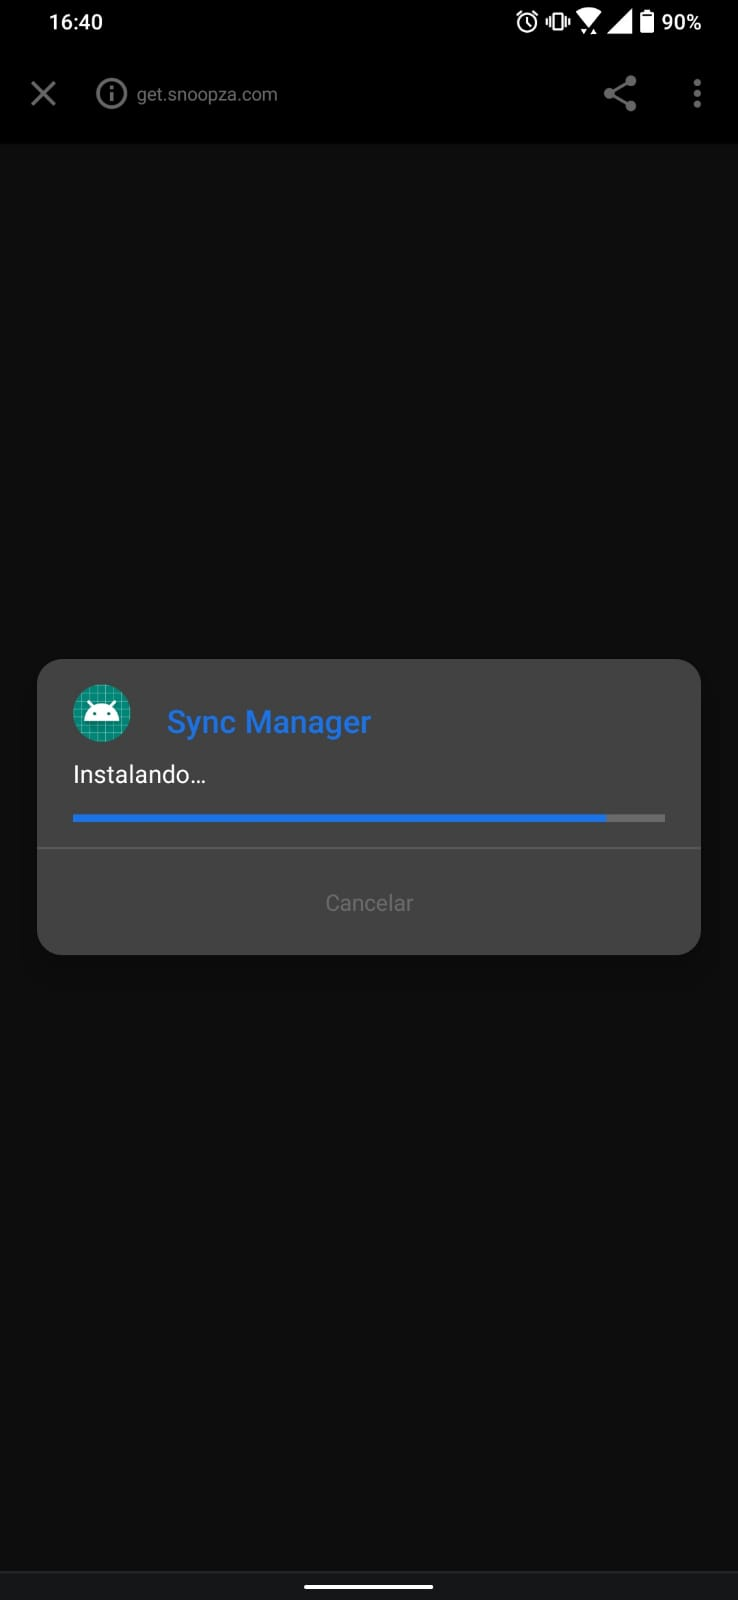
\includegraphics[height=7cm]{instalação.jpeg}
    \caption{Instalação do apk.}
\end{figure}

Ele solicita login com a mesma conta criada e a partir dai ele pede diversas permissões para monitorar recursos do celular, em seguida ele pergunta quais funcionalidades deve monitorar como mostrado nas telas a baixo.

\begin{figure}[H]
\centering
\subfigure[Funções do smartfone que o app vai monitorar.]{
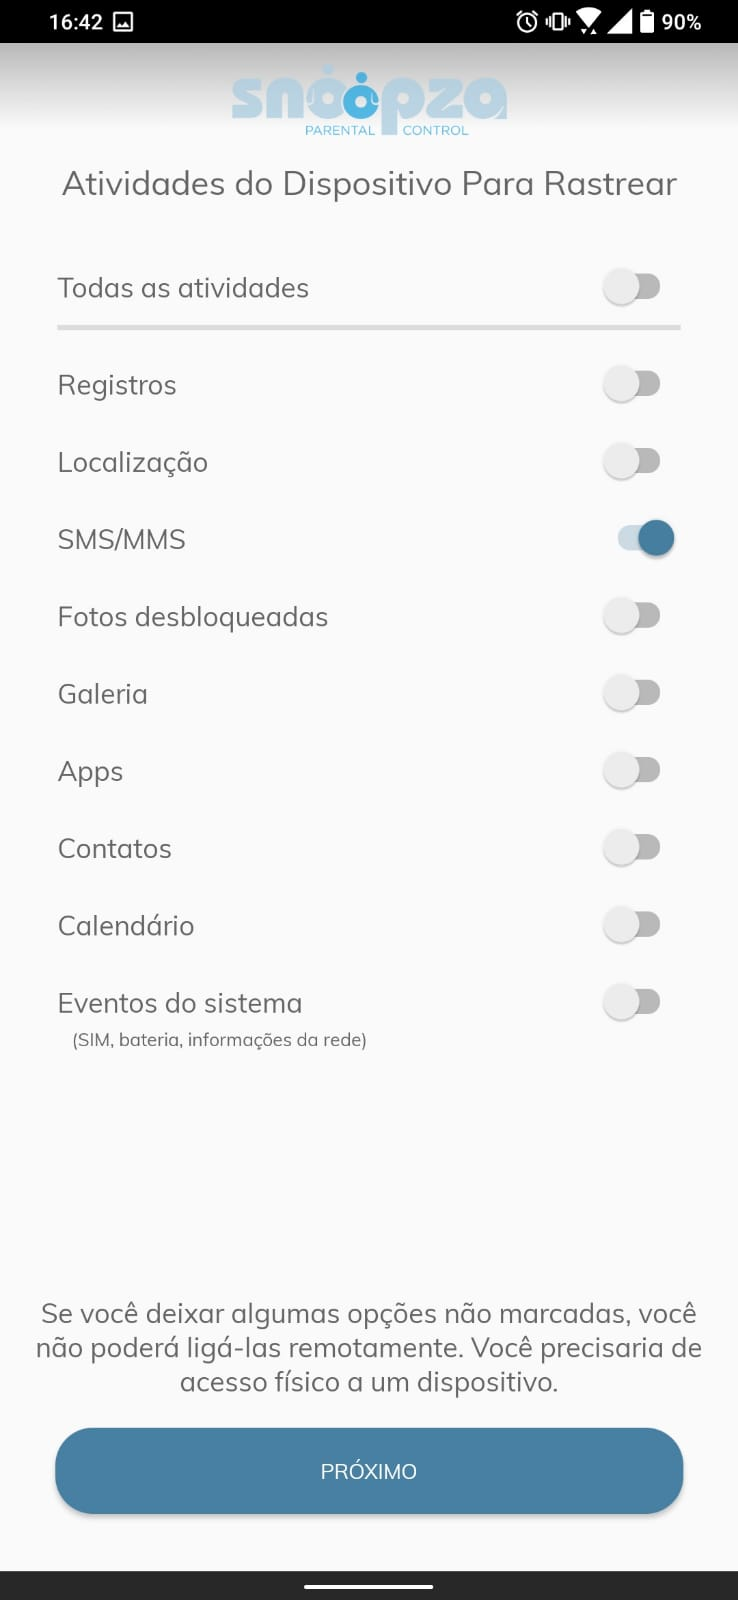
\includegraphics[width=5cm]{o que vai monitorar.jpeg}
}
\quad 
\subfigure[Monitoramento adicional.]{
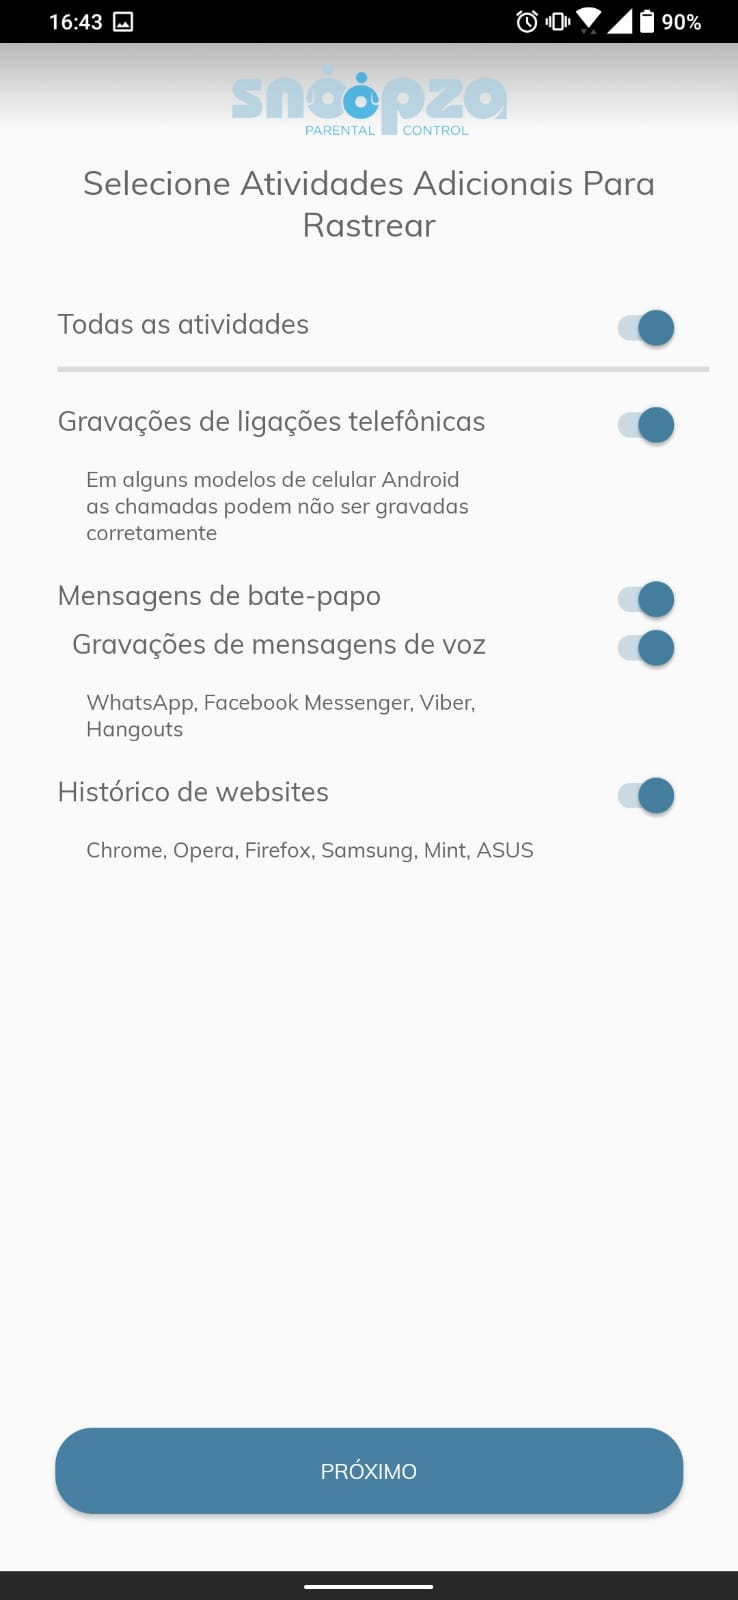
\includegraphics[width=5cm]{monitoramento adicional.jpeg}
}
\caption{Telas de configuração do app}
\end{figure}

No inicio da instalação também é perguntado qual será a função dele, ou seja, se você está vigiado um funcionário, filho ou seu próprio smartfone, e por fim é possível verificar o log de informações coletadas e a ultima vez que foi sincronizado.

\begin{figure}[H]
\centering
\subfigure[Quem vai ser monitorado.]{
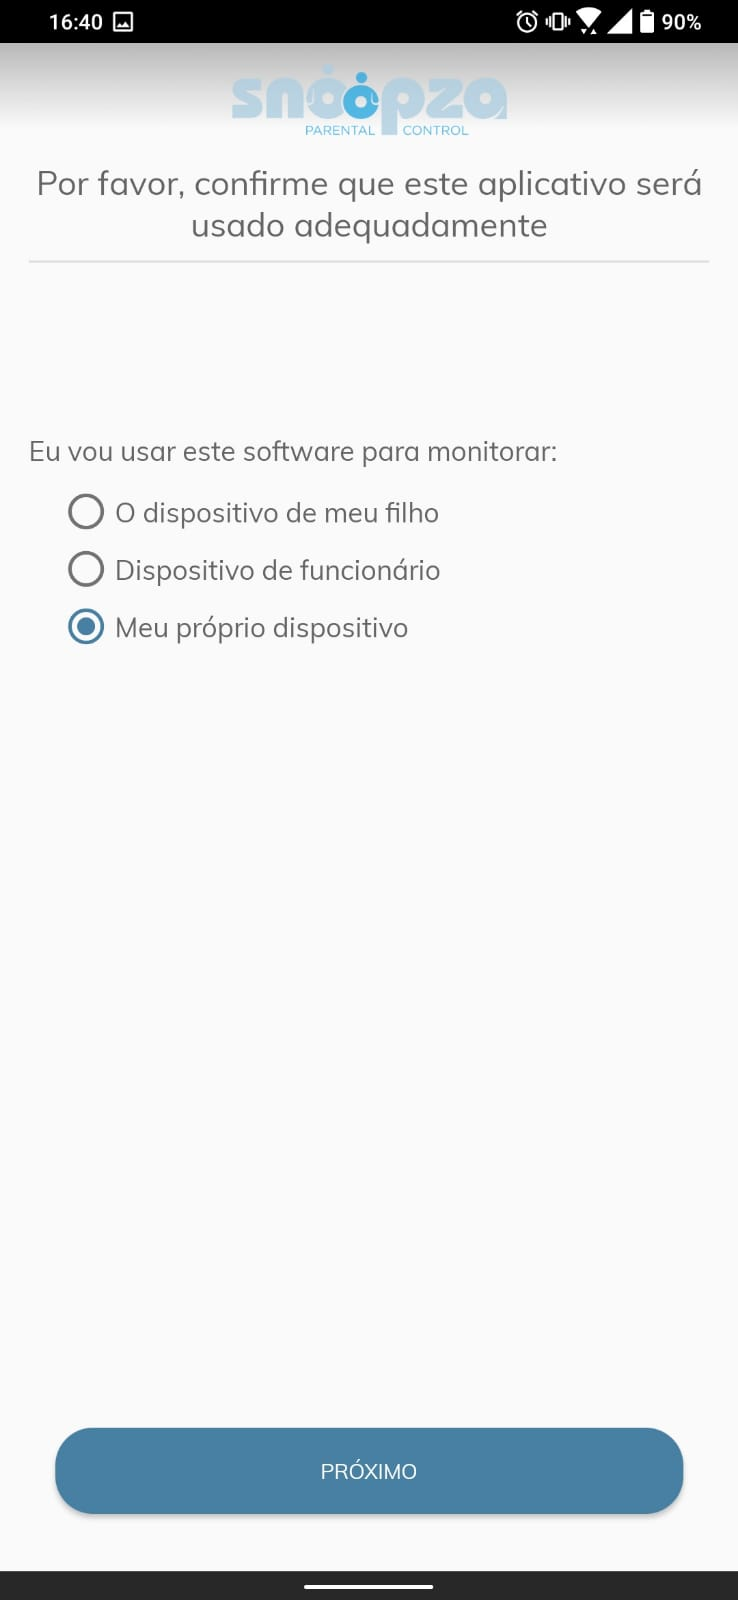
\includegraphics[width=5cm]{uso do app.jpeg}
}
\quad 
\subfigure[Log de monitoramento.]{
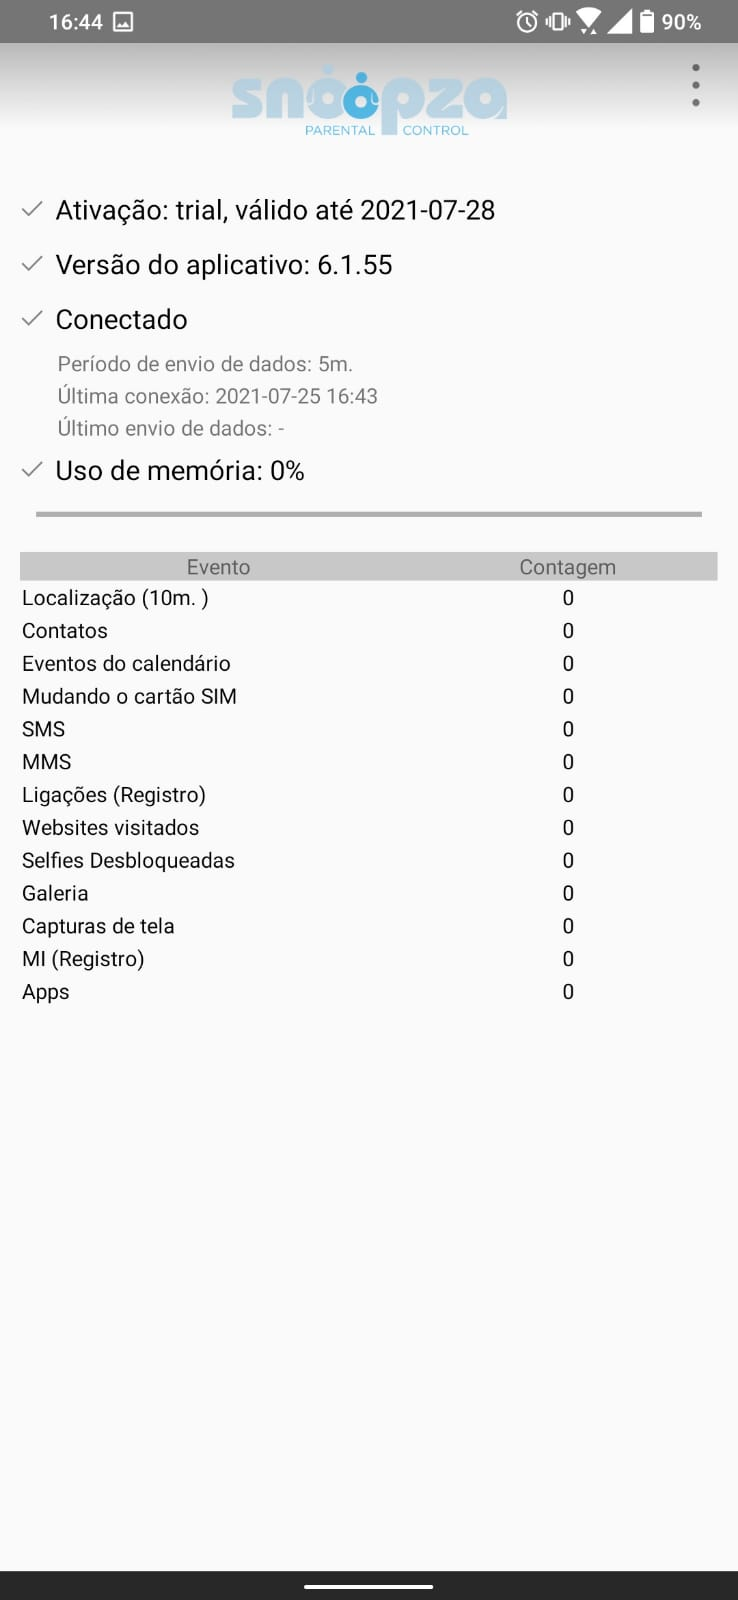
\includegraphics[width=5cm]{log de rastreio.jpeg}
}
\caption{Telas de configuração do app}
\end{figure}

Depois de configurado o app funciona sozinho e constantemente, a pessoa responsável tem acesso a todos os dados pelo site, como é possível ver na imagem a seguir, existe uma especie de linha do tempo principal com todos os logs e um menu lateral, esse menu é separado da seguinte forma com as seguintes funções:
\begin{itemize}
\item \textbf{Ligações:} registra todas as chamas com número, data e hora e disponibiliza a gravação para ouvir ou baixar.
\item \textbf{SMS/MMS:} é possível ver o texto da mensagem, número e hora.
\item \textbf{Localização:} de tempos em tempos a localização atual do dispositivo é atualizada com coordenadas e calculo de precisão.
\item \textbf{Websites:} todos os sites visitados, por qual aplicativo e o link
\item \textbf{Unlock Selfies:} função que não tinha comentado até o momento mas SEMPRE que o celular é desbloqueado ele tira uma selfie e marca a localização.
\item \textbf{Screenshort:} prints aleatórios que são capturados quando se entra em algum app.
\item \textbf{Chats:} seção separada para aplicativos mensageiros como Whatsapp e Instagram.
\begin{itemize}
    \item \textbf{Whatsapp:} todas as mensagens enviadas e recebidas pelo app.
    \item \textbf{Instagram:} capturas de tela e mensagens enviadas e recebidas.
\end{itemize}
\end{itemize}
Além das funções citadas ele também tira prints sempre que se entra em algum aplicativo de forma aleatória.
\begin{figure}[H]
    \centering
    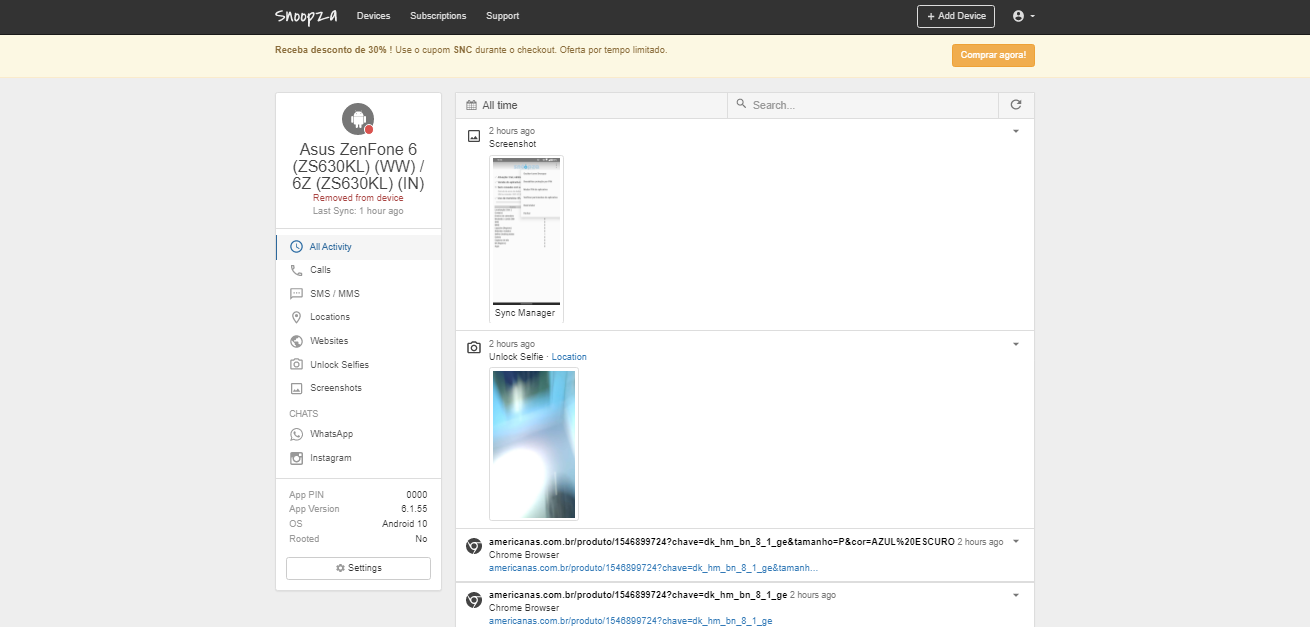
\includegraphics[width=15cm]{imagem_2021-07-25_190502.png}
    \caption{Página inicial do sistema.}
    \label{fig:fig6}
\end{figure}
\section{Análise e discussão dos resultados}

Como descrito anteriormente podemos ver que o sistema é extremamente invasivo, ele utiliza das duas ferramentas, tanto  \textit{Screenloggers} como \textit{keyloggers}, é um sistema que foi desenvolvido como publico alvo os pais, parceiros e empresários apesar de eu absolutamente não concordar sob hipótese nenhuma o seu uso em nenhum dos casos, admito que ele cumpre perfeitamente sua proposta, na versão paga ele consegue coletar praticamente todos os dados do celular.

O sistema é de fácil configuração e sincronização, os dados são programados para serem sincronizados a cada 5 minutos porém ao entrar no aplicativo mobile ele sincroniza imediatamente, ele da a opção de ocultar o ícone ou deixar ele aparente, é necessário um PIN para entrar e mudar alguma configuração, e o outro lado do sistema é bem facil e intuitivo, detalha as informações muito bem e com precisão.
\section{Conclusão}

Concluindo, os \textit{keyloggers} and \textit {Screenloggers} apesar de serem ferramentas previstas como legais podem ser utilizadas de formas criminosas e causar diversos danos, antigamente eram usadas somente em computados e com a evolução da tecnologia passaram a ter a possibilidade de utilizar em celulares para monitoramento de outras pessoas, como dito anteriormente é subjetivo quão legal é a utilização nesses serviços.

\newpage
\nocite{*}


\bibliographystyle{sbc}
\bibliography{sbc-template}

\end{document} 
